\documentclass[notes, 10pt]{beamer}
\usepackage{pgfpages}
\usetheme{Madrid}
\usepackage{lastpage}
\usepackage{appendixnumberbeamer}
\setbeameroption{hide notes}
%\setbeameroption{show notes on second screen =right}
\usepackage[us]{datetime}
\newdate{duedate}{9}{3}{2022} %to set a due date
\definecolor{UWRed}{RGB}{153,1,0}
\usecolortheme[named=UWRed]{structure}
\setbeamercolor{button}{bg=UWRed, fg=white}
\usepackage{appendixnumberbeamer}

\title{ECON 810 Final Project}
\date{\displaydate{duedate}}
\author{Yobin  \& Mitchell}
%\institute{}

\setbeamertemplate{footline}
{%
	\leavevmode%
	\hbox{\begin{beamercolorbox}[wd=.4\paperwidth,ht=2.5ex,dp=1.125ex,leftskip=.3cm,rightskip=.3cm]{frametitle}%
			
		\end{beamercolorbox}%
		\begin{beamercolorbox}[wd=.6\paperwidth,ht=2.5ex,dp=1.125ex,leftskip=.3cm,rightskip=.3cm plus1fil]{frametitle}%
			\usebeamerfont{section in head/foot}\insertshortauthor\hfill\insertframenumber/\pageref{mypage}
	\end{beamercolorbox}}%
	\vskip0pt%
}

\setbeamertemplate{footline}[frame number]

\newenvironment{wideitemize}{\itemize\addtolength{\itemsep}{10pt}}{\enditemize}
\newenvironment{wideenumerate}{\enumerate\addtolength{\itemsep}{10pt}}{\endenumerate}

\begin{document}
	\begin{frame}
		\maketitle
	\end{frame}

	\begin{frame}{Roadmap}
		\tableofcontents
	\end{frame}
	
	\section{Data}
	\begin{frame}{Data}
        \centering
        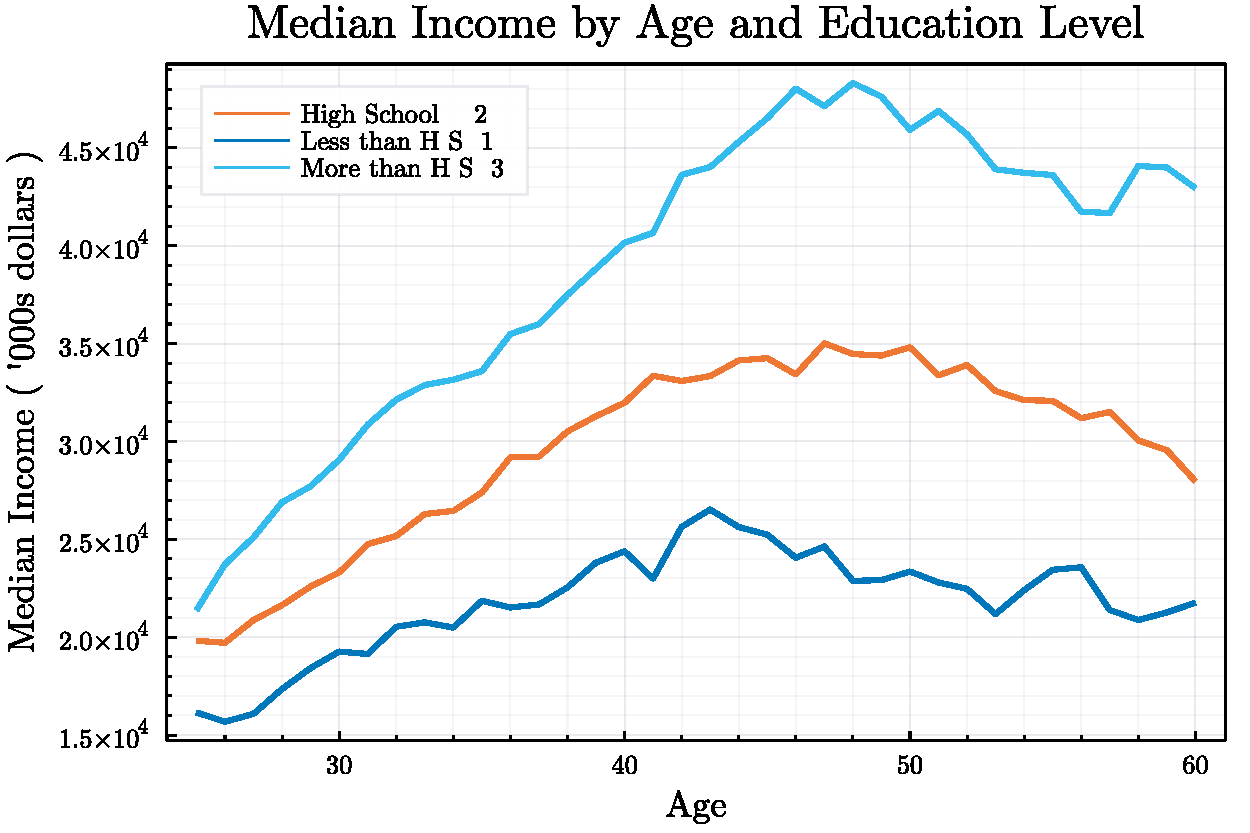
\includegraphics[width=12cm]{Figures/fig_median_income_by_age_and_education.pdf}
	\end{frame}
	\begin{frame}{Data}
        \centering
        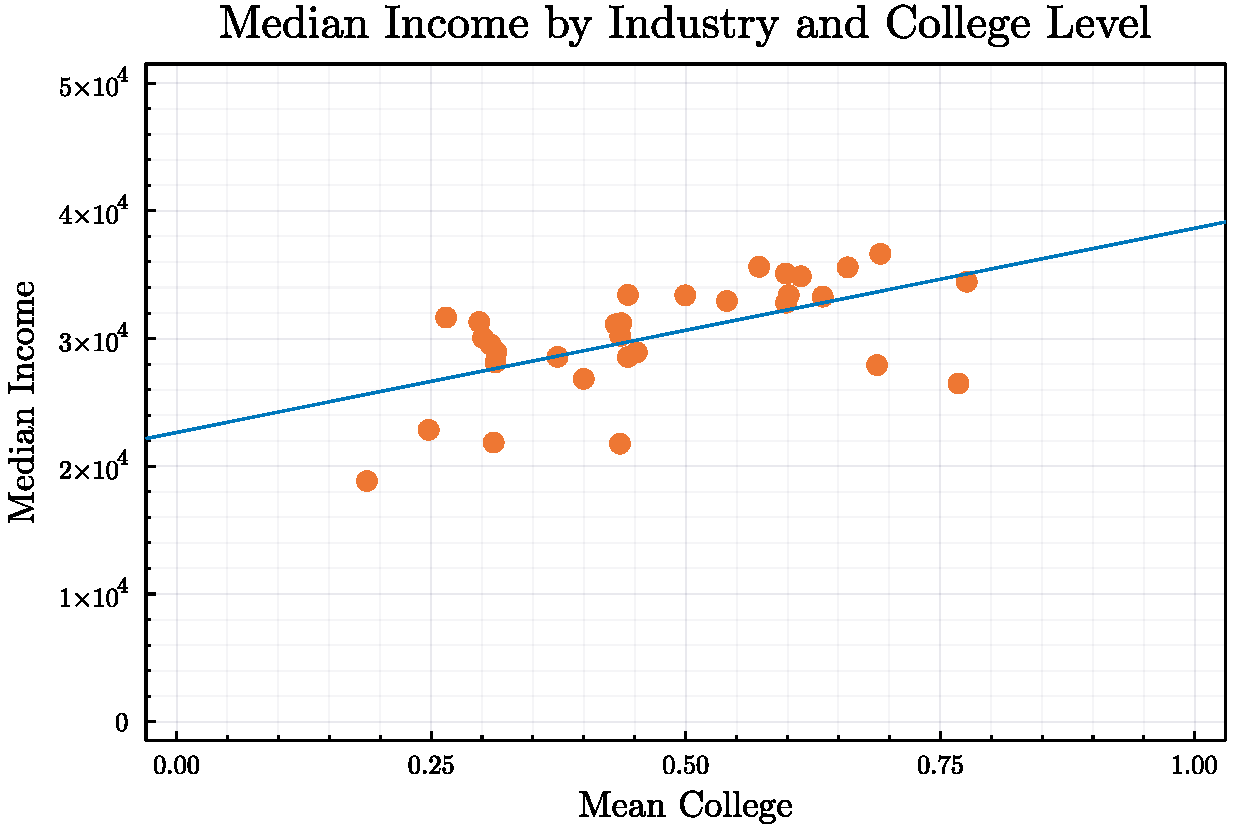
\includegraphics[width=12cm]{Figures/relation_median_wage_hs_percent.pdf}
	\end{frame}
	
	\section{Model}
	\begin{frame}{Model}{Environment}
		\begin{wideitemize}
			\item Agents live for $ T $ periods, without retirement. 
			\item Agents are heterogeneous in human capital $ h $, assets $ k $, and years of schooling $S$. 
			\item Agents have 1 unit of time endowment each period.
			\item They spend $ s \leq 1$ investing in education each period.
			\item Agents are either employed or unemployed (but looking for a job).
			\item There are two kinds of firms: good firms (high type) and bad firms (low type).
		\end{wideitemize}
	\end{frame}

	\begin{frame}[c]{Model}{Firms}
		\begin{wideitemize}
			\item There are $2$ firm types $I \in \{L,H\}$.
			\item $ \mu $ fraction of firms are low type.
			\begin{wideitemize}
				\item  Alternatively, we could think of this as $\mu$ proportion of all job vacancies are for the low type firm.
			\end{wideitemize}
			\item Firm type $I=L$ hires all workers while firm type $I=H$ hires only workers with $S \geq \underline{S}$.
			\item Firms differ in their productivity and consequently their rental rate of labor.
					\[  R_t^H > R_t^L, \forall t  \]
		\end{wideitemize}
	\end{frame}

	\begin{frame}{Model}{Workers}
		\begin{wideitemize}
			\item Workers are either employed (without on the job search) or unemployed (actively searching for a job).
			\item Agents take as given these $3$ state variables each period:
			\begin{wideitemize}
				\item $h \in \mathbb{R}_+$ human capital. Law of motion $ h' = \exp{z'} H(h,s) $.
				\item $k \in \mathbb{R}_+$ assets.
				\item $S \in \mathbb{R}_+$ (accumulated) schooling. Law of motion $ S' = S + s $.
			\end{wideitemize}
			\item $S$, i.e. years of schooling, determines the probability that an agents receives an offer from the high type firm. 
			\begin{wideitemize}
				\item We could think of $S$ as minimum required qualifications for a high paying job.
			\end{wideitemize}
		\end{wideitemize}
	\end{frame}

	\begin{frame}{Model}{Unemployed Agents}
		\begin{wideitemize}
			\item Agents divide their time between searching for a job with intensity $\gamma$ and schooling $s$: $$ \gamma + s = 1$$.
			\item Given $\gamma$ and $S$, their probability of finding a job is $$ \Pi_t(\gamma, S) = \gamma \cdot \frac{S}{t} $$.
			\item Value function depends on whether the agents have a minimum of $\underbar{S}$ years of schooling or not.
		\end{wideitemize}
	\end{frame}

	\begin{frame}{Model}{Unemployed Agents}
		\textbf{Value Function if $S < \underline{S}$}

		\begin{align*}
			U_t(h,k,S) =  \max_{k',s} \biggl\{ u(c) &+ \beta\mathbb{E}\biggl[\Pi(\gamma, S) \cdot \mu \cdot W^L_{t+1}(h',k',S')\\
			&+ (1 - \Pi(\gamma, S) \cdot \mu)U^L_{t+1}(h',k',S')  \biggr] \biggr\}
		\end{align*}


		\textbf{Value Function if $S \geq \underline{S}$}

		\begin{align*}
			U_t(h,k,S) = &  \max_{k',s} \biggl\{ u(c) + \beta\mathbb{E}\biggl[\Pi_t(\gamma, S) \left[\mu W^L_{t+1}(h',k',S') + (1 - \mu) W^H_{t+1}(h',k',S') \right]  \\
				+ & (1 - \Pi_t(\gamma, S)) U^L_{t+1}(h',k',S')  \biggr] \biggr\}
		\end{align*}
		with the budget constraint \[  c + k' \leq b + k(1+r). \]
	\end{frame}

	\begin{frame}{Model}{Employed Workers}
		\begin{wideitemize}
			\item Divide their time for $ s + l = 1 $.
			\item No on-the-job search allowed.
		\end{wideitemize}

		\vspace{0.5cm}
		
		\textbf{Value function, employed at firm $I$}
		\begin{align*}
			W^I_t(h,k,S) =  \max_{k',s} \left\{ u(c) + \beta\mathbb{E}\left[ (1 - \delta) W^I_{t+1}(h',k',S')
			+ \delta  U_{t+1}(h',k',S')  \right] \right\}
		\end{align*}
		with the budget constraint \[   c + k' \leq R^I_t h l + k(1 +r) \]
	\end{frame}

	\begin{frame}{Model}{Timing}
		\begin{wideenumerate}
			\item Start each period $t$ with $(k,h,S)$. At $t=1$, all agents are unemployed.
			\item Given their employment status at the start of each period, agents choose $s$ and $k'$, and pin down $c$.
			\item If employed, $l = 1 - s$. If unemployed, $\gamma = 1 - s$.
			\item If unemployed, given $\gamma, S$, agents have a probability of receiving a job offer.
			\item If $S > \underbar{S}$, of the offers they receive, a fraction $1 - \mu$ comes from high type firm.
			\item If employed, agents may lose their job with a probability $\delta$.
		\end{wideenumerate}
	\end{frame}
	
	\section{Results}
	\begin{frame}{Results}{}
		 \centering
        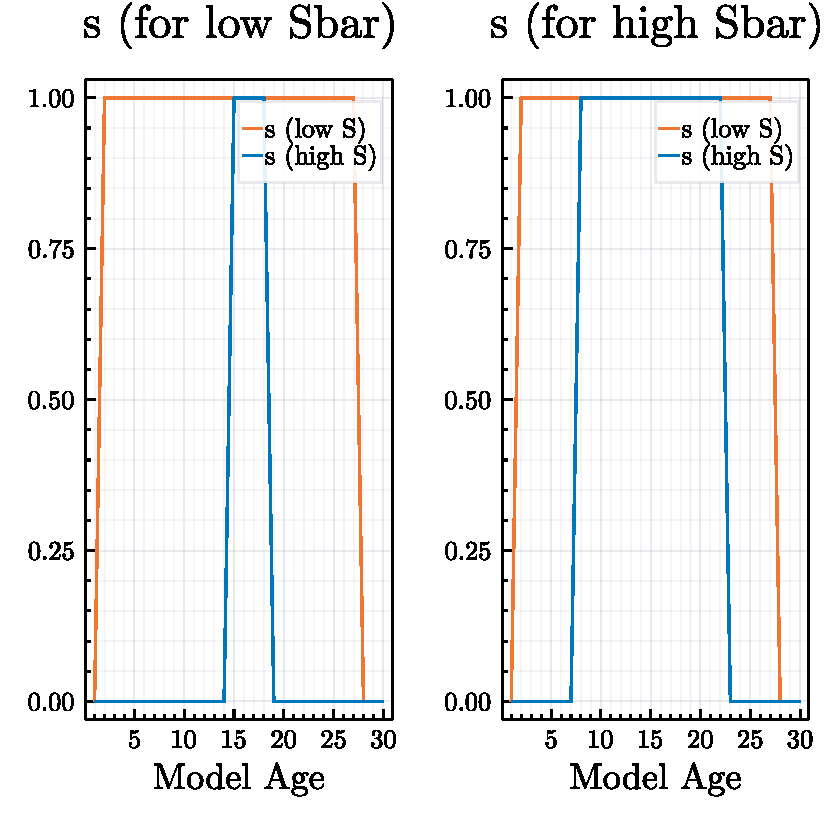
\includegraphics[width=12cm]{Figures/s_pol_U.pdf}
	\end{frame}

	\begin{frame}{Results}
        \centering
        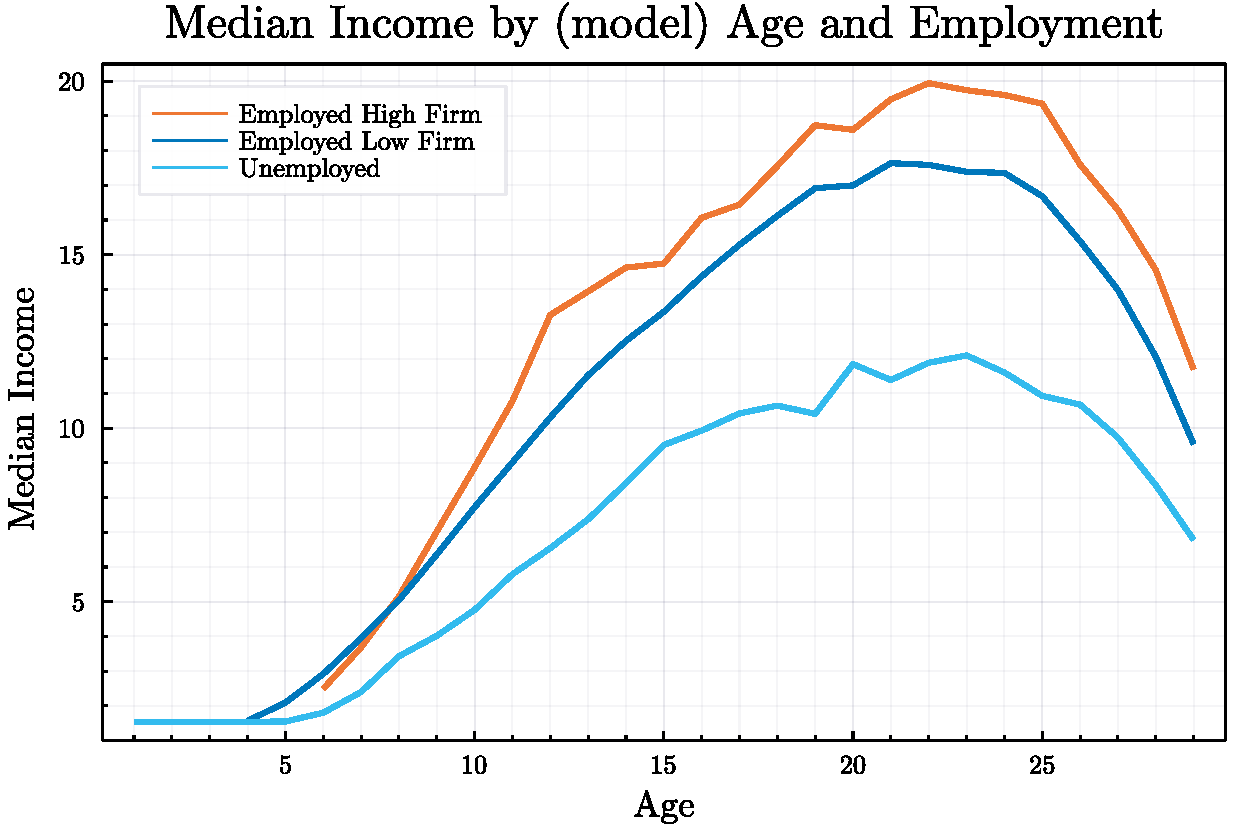
\includegraphics[width=12cm]{Figures/fig_median_income_by_age_and_employment_sim_data_v1.pdf}
	\end{frame}
	\begin{frame}{Results}
        \centering
        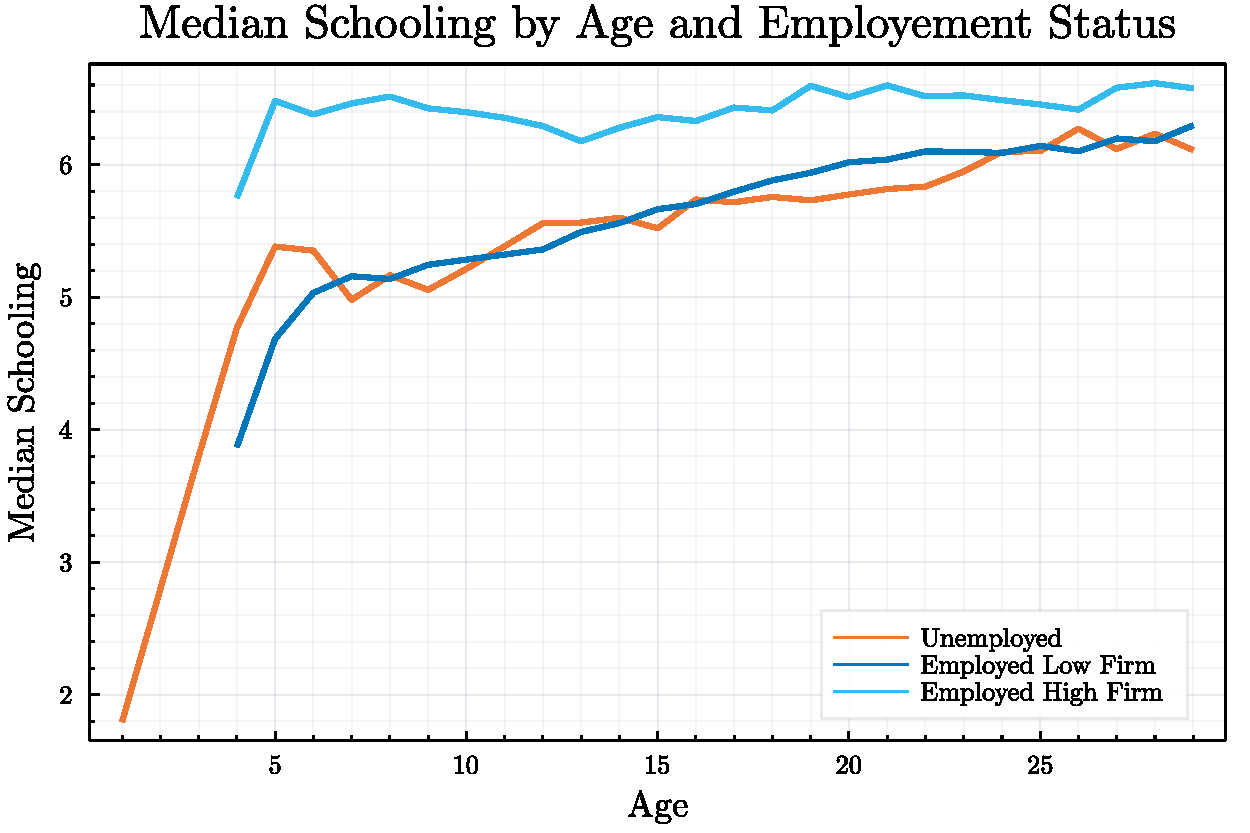
\includegraphics[width=12cm]{Figures/fig_median_income_by_age_and_employment_sim_data_v2.pdf}
	\end{frame}
    
	\begin{frame}{Results}
        \centering
        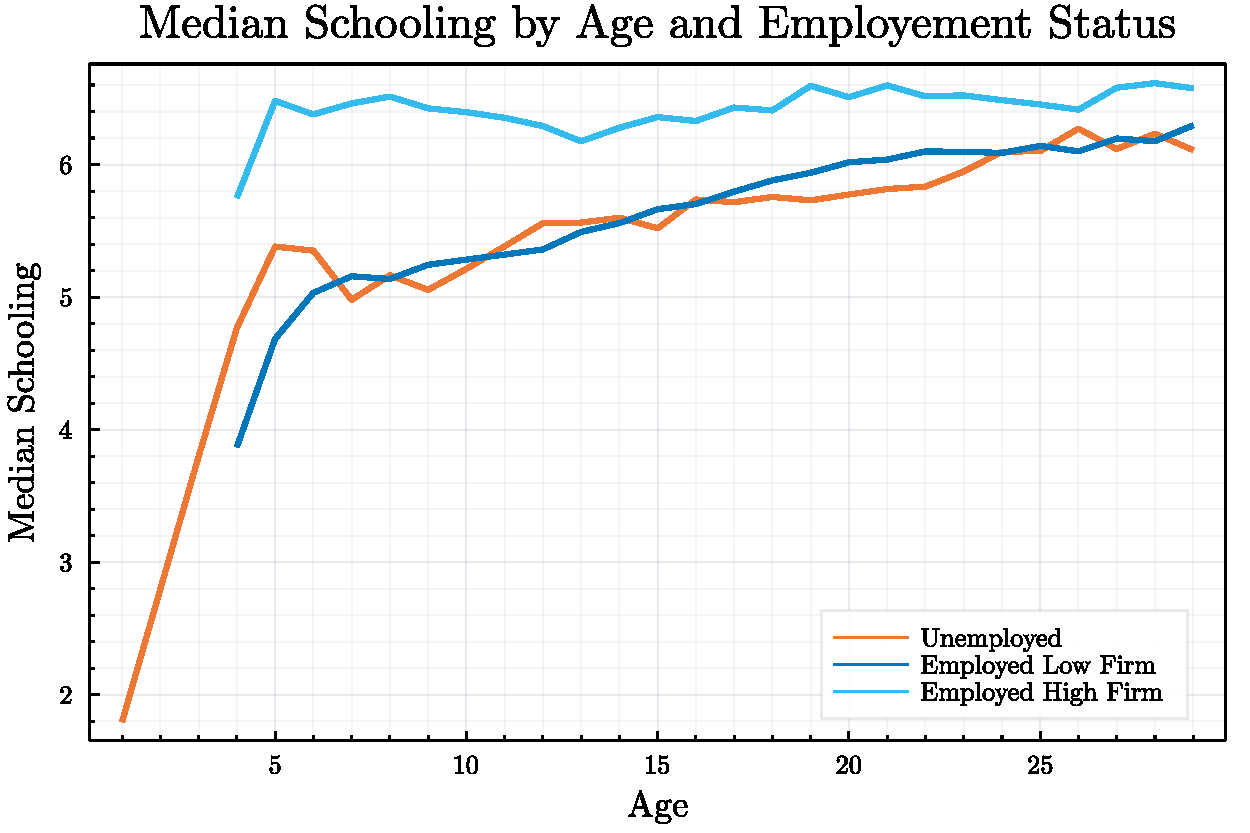
\includegraphics[width=12cm]{Figures/fig_median_schooling_by_age_and_employment_sim_data_v2.pdf}
	\end{frame}
\end{document}